\section{States, histories, occurrence geometry and evolution}\label{sec:objects}
This section fixes the objects, with the exact source of each definition. Notation is collected in Appendix~\ref{app:notation}.

\subsection{Generative states and histories}
\begin{definition}[source: Foundations Vol.~I; \Src{II}{def:select}, \Src{II}{def:history}]
For integers $m,N\ge1$ with $N\mid m$ write $m\xrightarrow{N}T_N(m)=m(N+1)^2/N$. A \emph{history} from the source $m_0$ is a word $w=(N_1,\dots,N_r)$ with $N_i\mid m_{i-1}$, $m_i=T_{N_i}(m_{i-1})$; its \emph{endpoint} is $\Endp(h)=m_r$, its \emph{content} is the multiset $c(h)\in\N^{A}$ of its letters. An adjacent transposition is \emph{legal} if both words are admissible; the \emph{swap graph} on the admissible arrangements of a fixed content has legal transpositions as edges, and its components are the \emph{swap classes}. The \emph{fibre sequence} of $h$ is $F(h)=(D(m_0),\dots,D(m_r))$.
\end{definition}
Since $m_i=m_{i-1}R(N_i)$ with $R(N)=(N+1)^2/N$, the endpoint is $\Endp(h)=m_0\prod_NR(N)^{c_N}$ and depends only on $(m_0,c)$.

\subsection{Collective states}
\begin{definition}[source: Foundations Vol.~II; \Src{III}{def:collective}]
For $x=a/b>0$ in lowest terms, $D(x)=\{d\ge2:d^2\mid a,\ d\equiv1\ (\mathrm{mod}\ b)\}$. If $D(x)\ne\emptyset$ put $L=\lcm D(x)$, $G=\gcd\{d-1\}$ and $C(x)=x+L^2/G$. For an integer $t$ the congruence is vacuous and $D(t)=\{d\ge2:d^2\mid t\}$.
\end{definition}
\begin{lemma}[occurrence monotonicity; \Src{III}{lem:M}]\label{lem:M-cited}
$D(x)\subseteq D(C(x))$. Hence along every orbit $x_n=C^n(x)$ the sets $D_n=D(x_n)$ are non-decreasing.
\end{lemma}

\subsection{Occurrence geometry}
\begin{definition}[the divisor-interval complex; \Src{III}{def:KD}, \Src{III}{thm:R3T1a}, \Src{III}{thm:A5T31}]
For a finite set $D\subset\Z_{\ge2}$ and $u,v\in D$ put $I(u,v)=\{z\in\Z:\gcd(u,v)\mid z\mid\lcm(u,v)\}$. The complex $K(D)$ has vertex set $D$, an edge $\{u,v\}$ iff $I(u,v)\cap(D\cup\{1\})=\{u,v\}$, and higher cells (cubical cells spanned by parallel edges) as in Paper~III. For a state $x$, $\Kmove(x)=K(D(x))$.
\end{definition}
By \Src{III}{thm:R3T1a}, the realised fibre, $\Kmove(x)$, its boundary maps, components and homology are functions of $D(x)$ alone. For an integer $t$, the active primes are those with $p^2\mid t$ and $\Kmove(t)$ is contractible \cite[\Src{III}{thm:B2T1}]{PaperIII}.

\subsection{Lattices and primitive relations}
For a state $x=a/b$ with active primes $p_1,\dots,p_k$ (those $p$ with $p^2\mid a$ and $p\nmid b$) let $\Lambda_b\subseteq\Z^k$ be the lattice of exponent vectors $\alpha$ with $\prod p_i^{\alpha_i}\equiv1\pmod b$, let $F$ be the fibre (its points in the box of admissible exponents, corresponding to $D(x)$) and $\Gr_q(x)$ the region Graver set: the primitive (conformally minimal) lattice vectors in the box. These are the objects of Paper~I; their transport under change of lattice is governed by \Src{I}{thm:P2T1} and \Src{I}{thm:P2T2}, abstract cells by \Src{I}{thm:cell-transport}, and the failure of laws one might expect by \Src{I}{thm:laws}.

\subsection{Factorization}
\begin{lemma}[factorization criterion]\label{lem:factor}
Let $\pi:X\to Y$ be surjective and $f:X\to Z$. Then $f=g\circ\pi$ for some $g$ iff $f$ is constant on every fibre of $\pi$; $g$ is then unique. If two points $x,x'$ have $\pi(x)=\pi(x')$ and $f(x)\ne f(x')$, no such $g$ exists.
\end{lemma}
\begin{proof}Define $g(y)=f(x)$ for any $x\in\pi^{-1}(y)$; well-definedness is constancy on fibres. The last statement is the contrapositive.\end{proof}
Throughout, an \emph{obstruction} to a factorization is a pair $x,x'$ as in the last sentence together with a proof that $\pi(x)=\pi(x')$ and $f(x)\neq f(x')$; its \emph{domain} is the set on which $\pi$ is taken (a fixed source, or all integers) and is stated each time.


\noindent\Cref{fig:states} shows arithmetic states and the objects attached to them.

\begin{figure}[t]\centering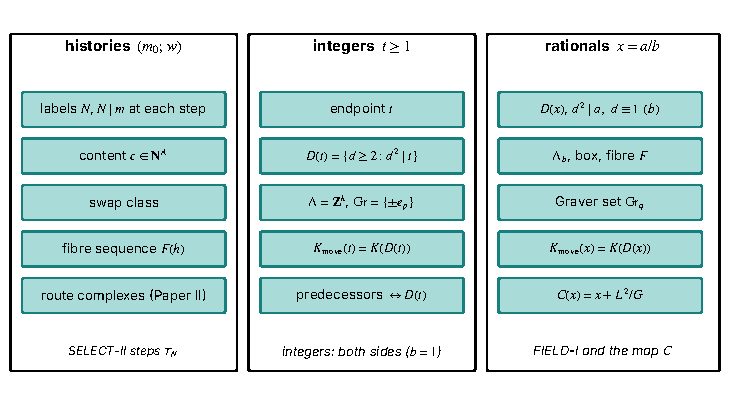
\includegraphics[width=\linewidth]{fig02_states_objects.pdf}
\caption{\textbf{Arithmetic states and the objects attached to them.} Three domains with their native constructions. Integers are the overlap: an integer is both an endpoint of histories and a collective state with denominator $1$. \emph{Schematic of domains.}}\label{fig:states}\end{figure}
